\documentclass{article}

\usepackage{fullpage}
\usepackage{color}
\usepackage{amsmath}
\usepackage{url}
\usepackage{verbatim}
\usepackage{graphicx}
\usepackage{parskip}
\usepackage{amssymb}
\usepackage{nicefrac}
\usepackage{listings} % For displaying code
\usepackage{algorithm2e} % pseudo-code

\title{Problem Definition}
\author{Peyman Bateni}

\usepackage{natbib}
\usepackage{graphicx}

\begin{document}

\maketitle

\section{Important Clarifications}
\begin{itemize}
    \item Is detection as defined by the BAA a multi-object task? If we are only focusing on placing bounding boxes on a single object in the image, then we may (with lots of emphasis on the may) need to update some assumptions.
\end{itemize}

\section{Important (Unconventional) Notes from BAA}
\begin{itemize}
    \item Goal is to make 6 orders of magnitude reduction in training data and 2 orders of magnitude reduction in data needed to adapt the model. Specific goals and milestones relative to the two phases (each consisting of 18 months) are provided in Figure \ref{goals}. For this work, we focus on object detection.
    \begin{figure}[t]
        \centering
        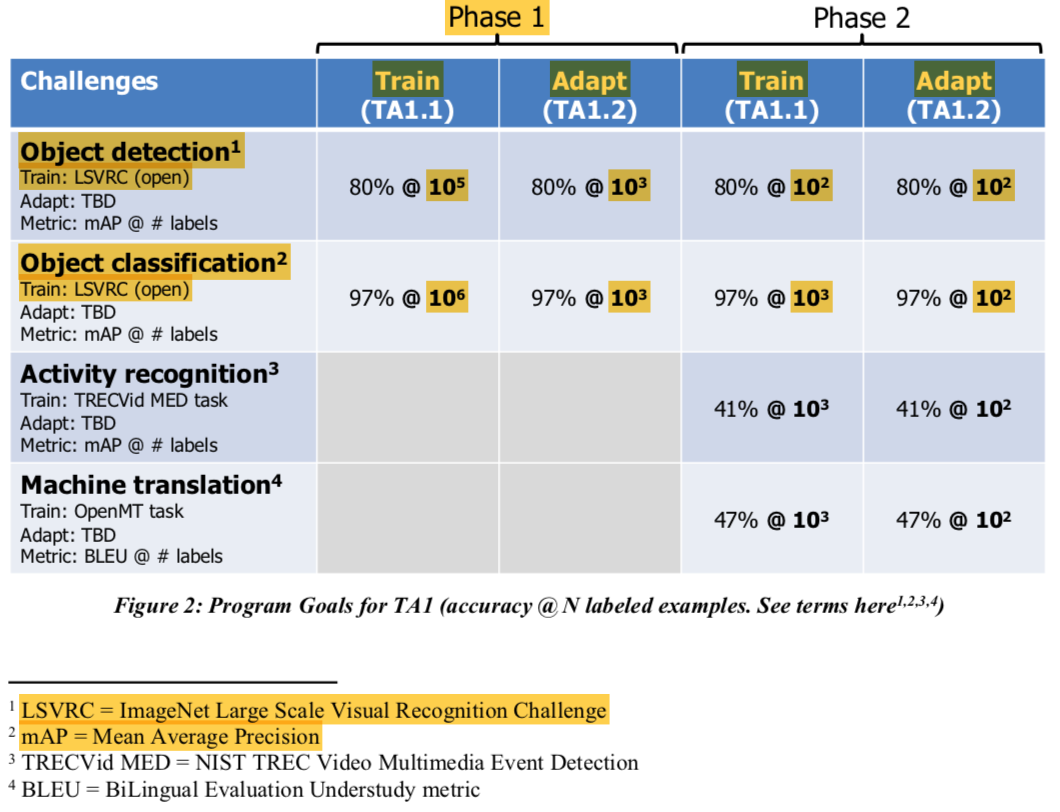
\includegraphics[width=6in]{Goals.png}
        \caption{DARPA goals and milestones defined on the four noted tasks.}
        \label{goals}
    \end{figure}[t]
    \item It's important to note that similar to other works in few-shot learning, we are able to leverage external publicly available dataset(s) or corpoa in enhancing performance. Additionally, it's noted that "[these] algorithms can make use of as much unlabeled data as they wish and they may choose specific examples for labeling". Thus, active learning is not only an option but seems to be encouraged throughout the BAA. It's not specified where the limit is drawn on amount on unlabeled data available but it's fair to be presumed to be orders of magnitude higher than the labeled amount.
\end{itemize}

\section{Problem Definition}
\begin{itemize}
        \item Assumptions for the classification case:
        \begin{itemize}
            \item $T_{source}^{train} = \{ (X_{1,1}, C_1), ... , (X_{n,1}, C_1), ... ,(X_{1,m}, C_m) , ... ,(X_{1,m}, C_m)\}$ where $X_{i,j}$ is the ith training example belonging to source class j, where $T_{source}^{train}$ consist of m class with n examples each with $n \ge 1000$ (NOTE: we set this last time but reviewing the LwLL description, I think this may be too high given the label limitations imposed).
            \item $T_{target}^{train} = \{ (X_{1,m+1}, C_m+1),...,(X_{k,m+1}, C_m+1), ..., (X_{1,m+h}, C_m+h),...(X_{k,m+h}, C_m+h) \}$ where we have k target classes with h examples each with $1 \leq k \leq 10$.
            \item $T_{zero-shot}^{train} = \{ C_{m+k+1}, ..., C_{m+k+d} \}$ defined the zero shot case where no examples are provided for the d zero-shot classes. While the notation allows for $T_{target}^{train}$ and $T_{zero-shot}^{train}$ to both be part of the problem definition, they are usually dealt with separately in the few-shot learning case (with d = 0) and the zero-shot learning case (with h = 0).
            \item At test time separate $T_{source}^{test}$ and  $T_{target}^{test}$ are provided although the number of examples per class in $T_{source}^{test}$ and $T_{target}^{test}$ may be different from that of $T_{source}^{train}$ and $T_{target}^{train}$ (ie. the assumption $n_{test} = n_{train}$ and $h_{test} = h_{train}$ doesn't necessarily hold). With that being said, the set distribution with respect to each class remains the same: $\forall C_i \in C, (\frac{card(T_{source,C_i}^{train})} {card(T_{source}^{train})} = \frac{card(T_{source,C_i}^{test})} {card(T_{source}^{test})}) \land (\frac{card(T_{target,C_i}^{train})} {card(T_{target}^{train})} = \frac{card(T_{target,C_i}^{test})} {card(T_{target}^{test})})$.
            \item $T_{zero-shot}^{test} = \{ (X_{1,m+k+1}, C_{m+k+1}) , ... , (X_{r,m+k+1}, C_{m+k+1}) , ... ,  (X_{1, m+k+d}, C_{m+k+d}) , ... , \\(X_{r, m+k+d}, C_{m+k+d}) \}$ at test time where $ 1 \le r \le 10$. Note that the zero-shot test set actually has examples, consisting of tuples as oppose to the set of only classes that's available during training.
            \item Assume for each class $C_i \in \mathbb{Z}$, with $1 \leq C_i \leq n+k+d$, there exists function $D: \mathbb{Z} \xrightarrow{} \Sigma^+$ such that (as per definition), $\Sigma = \{ "a", "b", "c", "d", ..., "z" \}$.
            \item Assuming the presence of a secondary source of class string label embeddings such as word2vec \cite{DBLP:journals/corr/MikolovSCCD13} or GLoVe embeddings \cite{pennington-etal-2014-glove}, there exists a function $J: \Sigma^{+} \xrightarrow{} \mathbb{R}^e$ where $e$ is the dimension of the embedding (often set to 50 or 100).
            \item \textbf{As suggested by the BAA, we also have acccess to $T_{unlabelled}^{train} = \{ X_{1}, X_{2}, ..., X_g \}}$ where $g \ge 10^{10}$. The assumption here is that we have near limitless unlabelled data for training. Additionally, there exists a function such that for $X_{i} \in \mathbb{Z}^{height,width}$ and corresponding class $C \in \mathbb{Z}$, $M: \mathbb{Z+}^{height \times width} \xrightarrow{} \mathbb{Z}$, providing the ability to request labels for unlabelled examples available. However, we can only use this function a total of $p$ times with $1 \leq p \leq 100$. Note that here, height and width are defined by the dimensions of the input image.
        \end{itemize}
        \item Assumptions for the detection case:
        \begin{itemize}
            \item Problem setting is somewhat similar with the addition of boundary boxes to each example/class topple in each of the sets. Changes would be as follows:
            \begin{itemize}
                \item $T_{source}^{train} = \{ (X_{1,1}, B_{1,1}, C_1), ... ,(X_{n,1}, B_{n,1}, C_1), ..., (X_{1,m}, B_{1,m}, C_m), ..., (X_{n,m}, B_{n,m}, C_m)\}$
                \item $T_{target}^{train} = \{ (X_{1,m+1}, B_{1,m+1}, C_m+1),...,(X_{k,m+1}, B_{k,m+1}, C_m+1),...,(X_{1,m+h}, B_{1,m+h}, C_m+h),...,(X_{k,m+h}, B_{k,m+h}, C_m+h) \}$
                \item where $B_{i,j}$ is an 8-tuple of positive pixel indices and $(0,0)$ is assumed to be the bottom left corner of the image.
            \end{itemize}
            \item The zero-shot training set remains the same with $T_{zero-shot}^{train} = \{ C_{m+k+1} ... C_{m+k+d} \}$. However, for the zero-shot test set, the set is update to include boundary boxes:
            \begin{itemize}
                \item $T_{zero-shot}^{test} = \{ (X_{1,m+k+1}, B_{1,m+k+1}, C_{m+k+1}), ... ,(X_{r,m+k+1}, B_{r,m+k+1},C_{m+k+1}), ... , \\(X_{1, m_k+d},B_{1, m_k+d}, C_{m+k+d}), ... , (X_{r, m_k+d},B_{r, m_k+d}, C_{m+k+d}) \}$
            \end{itemize}
            \item Similar functions $D$ and $J$ are present for mapping. \textbf{Additionally, $T_{unlabelled}^{train}$ and function $M$ are also available in the detection case. Note that here the examples are unlabelled meaning they don't have the boundary boxes either.}
            \item \textbf{For unlabelled example $X_{i} \in \mathbb{Z}^{height,width}$, there exists function $B: \mathbb{Z}^{height,width}$ \xrightarrow{} \mathbb{Z}^8}$ that maps the unlabelled image to an 8-tuple describing the boundary boxes. Similar to fucntion $M$, $B$ can only be used on a total of $p$ unlabelled images with $1 \leq p \leq 100$.
        \end{itemize}
        \item Distinctions to make for problems at hand (unless otherwise noted, definitions were taken from \cite{DBLP:journals/corr/Fu}):
        \begin{itemize}
            \item Few-shot learning:
            \begin{itemize}
                \item Parameter setting:
                \begin{itemize}
                    \item $n \ge 1000$ (you are given a reasonable number of examples per source class)
                    \item $1 \leq k \leq 10$ (on few-shot, otherwise known as target classes, you have a maximum of 10 examples per class)
                    \item Often $m > n$, although this is subject to the problem setting in the paper.
                    \item $d = 0$ (no zero-shot or zero example classes)
                \end{itemize}
                \item Performance is only based on classification/detection accuracy on $T_{target}^{test}$.
                \item Common jargon used includes N-way M-shot learning being defined as a few-shot learning task involving N target classes and M examples per target class.
            \end{itemize}
            \item Zero-shot learning:
            \begin{itemize}
                \item Parameter setting:
                \begin{itemize}
                    \item $n \ge 1000$ (you are given a reasonable number of examples per source class)
                    \item $k = 0$ (there are no target classes that have few examples)
                    \item $d > 0$ (there are $d$ zero-shot classes)
                \end{itemize}
                \item Performance is only based on classification/detection accuracy on $T_{zero-shot}^{test}$
                \item Similar notation is held with respect to N-way zero-shot learning specifying a zero-shot learning setting with N target classes.
            \end{itemize}
            \item Generalized few-Shot learning:
            \begin{itemize}
                \item Same parameter setting as few-shot learning
                \item Performance is based on classification/detection accuracy on both $T_{source}^{test}$ and $T_{target}^{test}$
            \end{itemize}
            \item Generalized zero-Shot learning:
            \begin{itemize}
                \item Same parameter setting as few-shot learning
                \item Performance is defined as classification/detection accuracy on both $T_{source}^{test}$ and $T_{zero-shot}^{test}$.
            \end{itemize}
            \item Open-set learning \cite{DBLP:journals/corr/geng2018}:
            \begin{itemize}
                \item With regards to few-shot learning and zero-shot learning respectively, openset learning defined the case where $h$ (ie. number of few-shot cases) in the first case and $d$ (ie. number of zero-shot cases) in the second case are not given (are unbounded at test time).
                \item Work here often involves label discovery as the network should be able to determine whether a presented example is of a previously seen class or new, for which in the latter case it must then learn a new class representation during test time, or effectively deal with it some other way.
            \end{itemize}
            \item Semi-supervised learning \cite{DBLP:journals/corr/boney2017}:
            \begin{itemize}
                \item In any of the aforementioned cases, problem would be defined as semi-supervised learning if we're given access to $T_{unlabelled}^{train}$ during training.
            \end{itemize}
            \item Active learning \cite{DBLP:journals/corr/boney2017}:
            \begin{itemize}
                \item Extension to the semi-supervised learning task where we are also given access to functions $M$ (and $B$ in the detection case) during training, thus allowing us to request labels for a limited ($\le100$) unlabelled examples.
                \item In the context of the DARPA project, this would be taking away from the number of starting labels (as the total number of labels used would be intended to be lower than the DARPA specified thresholds).
            \end{itemize}
        \end{itemize}
    \end{itemize}
    
\bibliographystyle{plain}
\bibliography{citations}
\end{document}
